\documentclass[letterpaper,10pt,conference]{ieeeconf}
\IEEEoverridecommandlockouts
\overrideIEEEmargins
\let\proof\relax
\let\endproof\relax
\usepackage{amsmath,amssymb,amsthm,mathtools}
\usepackage{graphicx,booktabs,array,cite}
\usepackage[hidelinks]{hyperref}

\newtheorem{assumption}{Assumption}
\newtheorem{proposition}{Proposition}
\newtheorem{lemma}{Lemma}
\newtheorem{theorem}{Theorem}
\newtheorem{corollary}{Corollary}

\newcommand{\Tp}{T_{\mathrm{p}}}
\newcommand{\Tn}{T_{\mathrm{n}}}
\newcommand{\rhoimp}{\rho_{\mathrm{imp}}}

\title{\LARGE\bf Snap-Load Transmission Between Cables Sharing a Towed Payload: Why the Impulsive Estimate Overpredicts}

\author{%
Hadi Hajieghrary$^{1}$ and Paul Schmitt$^{2}$%
\thanks{$^{1}$Hadi Hajieghrary (e-mail: \texttt{hadi.hajieghrary@gatech.edu}).}%
\thanks{$^{2}$Paul Schmitt (e-mail: \texttt{pauls@massrobotics.org, paul.schmitt@reynolds-moore.com}).}%
\thanks{The authors prepared this manuscript and present it solely in their individual capacities.}%
}

\begin{document}
\maketitle
\thispagestyle{empty}
\pagestyle{empty}

\begin{abstract}
When several robots or vessels tow a shared payload with cables, a re-engaging slack cable produces a snap load that can unload the neighboring cables. A natural rigid-impact (impulsive) estimate treats the re-engagement as instantaneous and holds the neighbors' far ends fixed. For a collinear tow of unilateral Kelvin--Voigt cables, we show that these assumptions require opposing mass regimes: brief contact requires light towing vehicles, whereas fixed far ends require heavy ones. We derive a similarity law under which the transmitted fraction of the snap peak is independent of closing speed and, without dissipation, of cable stiffness; an exact unloading criterion; and a closed-form law under a half-sine contact pulse which, with free far ends, lies at least 21\% below the corresponding impulsive value for up to ten cables. Nonlinear planar simulations of five controlled tugs in sixteen configurations test a forecast of 16.5\%, committed before any neighbor-tension drop was computed, against the rigid-impact 44\%. The pre-registered statistic stays well below the impulsive range in every configuration and rises with stiffness as predicted (by 3.6 against 4.5 percentage points), whereas a pre-registered pairwise test and a later fixed-dissipation control fail. A declared test at a second mass ratio supports the predicted rise (6.5 against 7.0 percentage points). Post hoc counterfactual re-integrations give a median transmission of 14.8\%; subtracting a time-shifted background drop instead gives a lower bound of 9.3\%. The rigid-impact baseline thus overstates cross-cable transmission roughly threefold.
\end{abstract}

\section{Introduction}\label{sec:intro}

Cable-connected teams let several robots or vessels move payloads that one vehicle could not, as in cooperative towing \cite{esposito2008cooperative, cheng2009cooperative, du2021cooperative}, multi-UAV transport \cite{sreenath2013dynamics, hajieghrary2026passive}, and cable-driven robots \cite{carricato2013stability}. Cables pull only while taut: a cable unloaded by payload oscillation, maneuvers, or disturbances snaps when pulled taut again, and because the cables share the payload, the snap changes every neighbor's tension; a neighbor that loses enough may go slack, letting slack spread.

We ask: \emph{given the peak load in a snapping cable, how much tension can a neighboring cable lose?} The answer is the cross-cable snap-transmission ratio, the largest reduction in a neighbor's tension divided by the snapping cable's peak. It links a fast transient to the tension margin that governs pretension selection, tension allocation, and slack screening. The natural estimate treats the re-engagement as an instantaneous impulse and holds the neighbors' far ends fixed. Yet the snap's duration and the neighbors' motion are set by the same stiffnesses and masses, so a consistent model must retain both finite contact and endpoint recoil. We take the snap peak as an input; predicting the snap itself, or a universal design bound, is not our aim.

Our contributions are the following.
\begin{enumerate}
    \item \textbf{Formulation and structural diagnosis.}
    We define the transmission ratio and, in the collinear model, an exact criterion for complete unloading of a neighbor. We show that the rigid-impact baseline needs light vehicles for an impulsive contact but heavy ones for held far ends; with free far ends and identical vehicles, the neighbor mode is never slower than the isolated-pair contact, so the impulsive regime is unreachable at every mass ratio.

    \item \textbf{Finite-duration transmission theory.}
    For a collinear tow of unilateral Kelvin--Voigt cables, a similarity law makes the ratio independent of closing speed and, without dissipation, of stiffness. Under a half-sine contact pulse the ratio is closed-form in mass ratio and cable count and, with free far ends, at least 21\% below the corresponding impulsive value for up to ten cables. Self-consistent contact is treated numerically.

    \item \textbf{Evaluation in a nonlinear controlled fleet.}
    A planar simulation of five controlled tugs in sixteen configurations is scored against a forecast committed before any neighbor-tension drop was computed, and a later declared test adds a second vessel mass. The evidence, summarized in Table~\ref{tab:evidence_status}, supports the predicted population-level magnitude and parameter dependence, not a pairwise distribution or a universal bound.
\end{enumerate}

\section{Related Work}
\label{sec:related}

Nonsmooth mechanics represents a newly active unilateral constraint by an impulse and a velocity jump; the Delassus operator, the inverse inertia seen by the constraints, maps constraint impulses to velocity changes~\cite{moreau1988unilateral,brogliato2016nonsmooth}, and appears in robotics as the inverse operational-space inertia~\cite{khatib1995inertial}. Compliant-impact theory shows that the outcome can instead depend on relative stiffnesses and stored energy~\cite{liu2008frictionless}, and impact-aware planning treats the slack--taut transition of a cable-suspended aerial robot as a hybrid impact event~\cite{wang2024impactaware}. None of these determines the peak unloading of one cable when another re-engages through a shared movable payload; we use the rigid-impact construction only as a baseline.

Marine snap-loading work focuses on the force \emph{within the snapping line}: the dimensionless snap susceptibility of a package suspended from multiple cables~\cite{niedzwecki1991snap}, lumped slack--taut cable dynamics~\cite{huang1993numerical}, continuous cables coupled through a submerged body and deck machinery~\cite{hann1995multicable}, first-snap forces in synthetic ropes~\cite{hennessey2005experimental}, extreme mooring tensions in slack--taut events~\cite{hsu2017snap,hann2015snatch,qiao2020snap}, and finite-element and discontinuous-Galerkin models that resolve axial waves~\cite{palm2017hpadaptive}. These models are far richer than our lumped one, but none, including the multi-cable formulation of~\cite{hann1995multicable}, defines the normalized peak transfer from a snapping cable to a neighbor or asks how freely moving endpoints alter it.

Cooperative transport research models several cables on a movable payload to address equilibrium, feasible tensions, trajectories, and manipulation~\cite{michael2009cooperative,sreenath2013dynamics}, or towing-force allocation under disturbances~\cite{du2021cooperative}, to keep transport feasible rather than to quantify the transient transmitted between cables.

\section{Model and Problem}\label{sec:model}

\subsection{The Fleet and the Question}
A fleet of $N$ vessels tows one payload, each through one cable loaded to the pretension $T_0$ in steady tow. The cables are unilateral Kelvin--Voigt lines, with tension $[k e_i+c\dot e_i]_+$ for elongation $e_i>0$ and none otherwise \cite{hall2015validation}; the clamp keeps the damper from pushing in compression just before separation \cite{hunt1975coefficient}. When cable $j$ re-engages with closing speed $V=\dot e_j(0^+)>0$, its tension reaches $\Tp$ and returns to zero after a finite contact. We call this a \emph{snap} (Fig.~\ref{fig:fleetsnap}) and define the transmission to neighbor $i$ by
\begin{equation}\label{eq:rho}
  \rho_{ij}=\frac{\max_t\Delta T_i(t)}{\Tp},\qquad \Tp=\max_t T_j(t),
\end{equation}
where $\Delta T_i$ is the drop relative to the counterfactual tension without the snap. Section~\ref{subsec:magnitude} realizes the counterfactual numerically.

\begin{figure}[t]
  \centering
  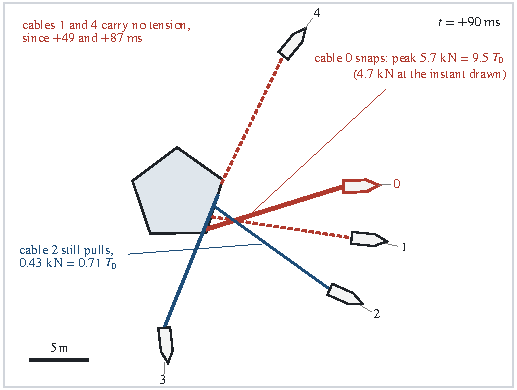
\includegraphics[width=\columnwidth]{fig_fleet_snap}
  \caption{A selected, atypical snap on the testbed ($T_0=0.6$\,kN), $90$\,ms after cable~0 re-engages; taut cables solid (width growing with tension), slack cables dashed. Cable~0 peaks at $9.51T_0$, far above the scored range $[T_0,4T_0]$, at $58$\,ms. Cable~1, already near slack ($0.66T_0$), reaches zero at $49$\,ms; cables 4 and 3 follow at $87$ and $206$\,ms; cable~2 stays taut for one engagement period.}
  \label{fig:fleetsnap}
\end{figure}

\subsection{Collinear Reduction}
Section~\ref{sec:test} measures the cost of the following idealization on a planar fleet.
\begin{assumption}\label{ass:collinear}
The cables are parallel and attached so a snap does not rotate the payload; all have stiffness $k$ and damping $c$, the vessels share mass $m_A$ and drag $c_A$, and the payload has mass $m_L$ and drag $c_L$. During one snap, thrust and weather forces are constant, so they cancel in the perturbation about the steady tow, and the $N-1$ neighbors begin from a common taut state of tension $\Tn>0$.
\end{assumption}
Let $x$, $y_j$, and $y$ be payload, parent-vessel, and neighbor-vessel displacements from steady tow; by symmetry and uniqueness the neighbors move together.
\begin{assumption}\label{ass:wellposed}
Solutions cross the switching surface $e_j=0$ transversally, so the hybrid solution is unique.
\end{assumption}
While the neighbors remain taut,
\begin{equation}\label{eq:model}
\begin{aligned}
  m_L\ddot x &= f+(N-1)\delta T-c_L\dot x,\\
  m_A\ddot y &= -\delta T-c_A\dot y,\\
  m_A\ddot y_j &= -f-c_A\dot y_j,
\end{aligned}
\end{equation}
with $\delta T=k(y-x)+c(\dot y-\dot x)$, $f=[ke_j+c\dot e_j]_+$ for $e_j=y_j-x>0$ and $f=0$ otherwise, and zero initial state except $\dot y_j(0)=V$. Hence $\Delta T=-\delta T$ and $\rho=\max\Delta T/\max f$ over the first contact and its response; a later contact of cable $j$ is a new snap. For prescribed $f$, \eqref{eq:model} is linear, so the snap contribution is a superposed perturbation; the nonlinear planar testbed instead uses paired re-integrations with and without the snapping-cable force, a counterfactual rather than a superposition.

\subsection{The Impulsive Estimate}
Replace the contact by an impulse $J=\int f\,dt$, hold the neighbor vessels ($y\equiv0$), and ignore dissipation. The payload leaves with velocity $J/m_L$ and oscillates at $\omega_L=\sqrt{(N-1)k/m_L}$, giving $\max\Delta T=kJ/(m_L\omega_L)$. For an isolated half-sine contact $f=\Tp\sin\omega_e t$ on $[0,\pi/\omega_e]$, with $\omega_e=\sqrt{k(1/m_A+1/m_L)}$, $J=2\Tp/\omega_e$ and
\begin{equation}\label{eq:imp}
  \rhoimp=\frac{2k}{m_L\omega_L\omega_e}.
\end{equation}
Equivalently, $\rhoimp=(2k/(\omega_L\omega_e))\,[W^\top M_L^{-1}W]_{ij}$, where $W$ has the cable wrenches $(d_i,r_i\times d_i)$ as columns, with unit chord $d_i$ and attachment arm $r_i$, and $M_L=\operatorname{diag}(m_L,m_L,I_L)$; under Assumption~\ref{ass:collinear} the lever arms vanish and the off-diagonal entry is $1/m_L$.
At $N=5$ and $m_A/m_L=0.24$, \eqref{eq:imp} gives $\rhoimp=0.440$, so a neighbor at $T_0$ would unload near $2.3T_0$. It is the direct impact construction, not a published law; we use it as the baseline and remove its finite-contact and held-end assumptions below.

\section{Transmission Theory}\label{sec:theory}

\subsection{Similarity and Threshold Laws}\label{sec:similarity}

\begin{proposition}\label{prop:similarity}
Let Assumptions~\ref{ass:collinear} and~\ref{ass:wellposed} hold and let the neighbors remain taut. Define $\gamma = c/\sqrt{k m_L}$, $\gamma_L = c_L/\sqrt{k m_L}$ and $\gamma_A = c_A/\sqrt{k m_L}$. Every tension in \eqref{eq:model} equals $V\sqrt{k m_L}$ times a function of $t\sqrt{k/m_L}$ that depends only on $m_A/m_L$, $N$, $\gamma$, $\gamma_L$ and $\gamma_A$. Consequently $\rho=\Phi(m_A/m_L,N,\gamma,\gamma_L,\gamma_A)$ for a function $\Phi$ that does not depend on $V$, $k$ or $\Tn$ separately, and without dissipation $\rho$ depends on $m_A/m_L$ and $N$ alone.
\end{proposition}

\begin{proof}
Set $\ell=V\sqrt{m_L/k}$ and $s=t\sqrt{k/m_L}$, with $x=\ell\xi$, $y=\ell\eta$, and $y_j=\ell\eta_j$. Inertial, spring, and damping terms in \eqref{eq:model} share the force scale $k\ell=V\sqrt{k m_L}$; after division by it, the equations and switching surface depend only on $r=m_A/m_L$, $N$, $\gamma$, $\gamma_L$, and $\gamma_A$, with $\eta_j'(0)=1$. Uniqueness fixes the corresponding dimensionless response. Since both $f$ and $\delta T$ scale by $k\ell$, their peak ratio has the stated dependence, and $\Tn$ does not enter \eqref{eq:model}.
\end{proof}

Without solving \eqref{eq:model}, the proposition predicts that stiffness can change the transmission only through the three dissipation numbers, which fall as $k^{-1/2}$; an undamped law such as \eqref{eq:imp} cannot depend on stiffness at all (tested in Section~\ref{sec:stiffness}). The same scaling gives an exact criterion for slackening a neighbor, that is, for its tension to reach zero. Let $\bar T_{\mathrm p}$ denote the peak that the taut model \eqref{eq:model} assigns to a given closing speed; it equals the actual peak whenever the neighbors stay taut.

\begin{corollary}\label{cor:threshold}
Under Assumptions~\ref{ass:collinear} and~\ref{ass:wellposed}, a snap slackens the neighbors if and only if $\rho\,\bar T_{\mathrm p}\ge\Tn$.
\end{corollary}

\begin{proof}
The minimum taut-model tension is $\Tn-\rho\bar T_{\mathrm p}$. If positive, uniqueness keeps the actual solution taut. Otherwise, the actual and taut solutions coincide until the first zero of $\Tn+\delta T$, so the neighbor reaches zero tension.
\end{proof}

\noindent\textit{Control implication.}
Since $\Tn$ does not enter \eqref{eq:model}, the proof extends to unequal pretensions $T_{\mathrm{n},i}$: no neighbor slackens if and only if $\rho\,\bar T_{\mathrm p}<\min_i T_{\mathrm{n},i}$. The bound is joint, since once a weaker neighbor slackens the others unload further, so a pretension or allocation policy must enforce it for all neighbors at once, with $\bar T_{\mathrm p}\propto V$ predicted from the anticipated closing speed (Proposition~\ref{prop:similarity}) and a margin for model error.

\subsection{Closed Form Under the Contact Pulse}\label{sec:closedform}

To obtain $\rho$ in closed form, we replace the self-consistent contact by the isolated-pair pulse of \eqref{eq:imp} and set aside dissipation; Sections~\ref{sec:selfconsistent} and~\ref{sec:dissipation} restore both. The ratio of the peak half-sine response of a linear oscillator to its impulsive response is the pulse's shock spectrum \cite{harris2002shock}; we need it with an argument that identifies which extremum is the peak.

\begin{lemma}\label{lem:spectrum}
Let $0<\varepsilon\le 3$ and let $u$ solve $\ddot u+\varepsilon^2u=\sin t$ on $[0,\pi]$ and $\ddot u+\varepsilon^2u=0$ afterwards, with $u(0)=\dot u(0)=0$. Then $\sup_{t\ge0}|u(t)| = 2S(\varepsilon)/\varepsilon$, where
\begin{equation}\label{eq:spectrum}
  S(\varepsilon) =
  \begin{cases}
    \dfrac{\cos(\pi\varepsilon/2)}{1-\varepsilon^2}, & \varepsilon<1,\\[4pt]
    \pi/4, & \varepsilon = 1,\\[2pt]
    \dfrac{\sin\!\big(2\pi/(1+\varepsilon)\big)}{2(\varepsilon-1)}, & 1<\varepsilon\le 3.
  \end{cases}
\end{equation}
Moreover $S(\varepsilon)\to1$ as $\varepsilon\to0$, and $S$ decreases on $[1,3]$ from $\pi/4$ to $1/4$.
\end{lemma}

Since the same impulse, $\int_0^\pi\sin t\,dt=2$, applied at $t=0$ gives amplitude $2/\varepsilon$, $S$ is the peak relative to the impulsive one.

\begin{proof}
For $\varepsilon\neq1$,
\begin{equation*}
 u=\frac{\sin\varepsilon t-\varepsilon\sin t}{\varepsilon(1-\varepsilon^2)},\qquad
 \dot u=\frac{2\sin\frac{(1+\varepsilon)t}{2}\sin\frac{(1-\varepsilon)t}{2}}{1-\varepsilon^2}.
\end{equation*}
The energy $E=u^2+\dot u^2/\varepsilon^2$ satisfies $\dot E=2\dot u\sin t/\varepsilon^2$ on $[0,\pi]$, is constant afterwards, and bounds $|u|\le\sqrt E$. For $\varepsilon<1$, both sine factors are positive on $(0,\pi]$, so $\dot u>0$, $E$ is nondecreasing, and the supremum is $\sqrt{E(\pi)}$. For $1<\varepsilon\le3$, $\sin((\varepsilon-1)t/2)>0$ on $(0,\pi)$, while $\sin((1+\varepsilon)t/2)$ is positive before $t^*=2\pi/(1+\varepsilon)$ and, because $(1+\varepsilon)\pi/2\le2\pi$, nonpositive on $[t^*,\pi]$; hence $u$ increases to $t^*$, $E$ is nonincreasing afterwards, and $|u(t)|\le\sqrt{E(t^*)}=u(t^*)=\sin t^*/(\varepsilon(\varepsilon-1))$ for $t\ge t^*$, using $\varepsilon t^*=2\pi-t^*$. At $\varepsilon=1$, $u=(\sin t-t\cos t)/2$ with $\dot u=(t\sin t)/2\ge0$, so the supremum is $\sqrt{E(\pi)}=\pi/2$. Dividing by $2/\varepsilon$ gives \eqref{eq:spectrum}. On $(1,3]$, $w=\pi-t^*\in(0,\pi/2]$ increases with $\varepsilon$ and $S=(\pi-w)\sin w/(4w)$, whose $w$-derivative has the sign of $w(\pi-w)\cos w-\pi\sin w<0$, since $\pi\sin w\ge\pi w\cos w>(\pi-w)w\cos w$ for $\cos w>0$ and the first term vanishes at $w=\pi/2$.
\end{proof}

\begin{theorem}\label{thm:closedform}
Let Assumption~\ref{ass:collinear} hold with $c=c_L=c_A=0$, and replace the contact force in \eqref{eq:model} by $f(t)=\Tp\sin\omega_e t$ on $[0,\pi/\omega_e]$ and $f=0$ afterwards. Let $\omega_q=\omega_L$ if the neighbor vessels are held and $\omega_q=\omega_f\coloneqq\sqrt{k((N-1)/m_L+1/m_A)}$ if they are free. If $\varepsilon_q\coloneqq\omega_q/\omega_e\le3$, then
\begin{equation}\label{eq:closedform}
  \rho = \frac{2k}{m_L\,\omega_q\,\omega_e}\,S(\varepsilon_q).
\end{equation}
\end{theorem}

\begin{proof}
For $q=x-y$, \eqref{eq:model} gives $\ddot q+\omega_q^2q=f/m_L$ (with $q=x$ when held) and $\Delta T=kq$. Setting $s=\omega_e t$ and $q=\Tp u(s)/(m_L\omega_e^2)$ reduces the response to Lemma~\ref{lem:spectrum}, yielding \eqref{eq:closedform}.
\end{proof}

The prefactor in \eqref{eq:closedform} is the impulsive transmission of the same fleet, and \eqref{eq:imp} is the held case with $S=1$. With free far ends and $N\le10$, the theorem holds for every choice of masses:

\begin{corollary}\label{cor:unreachable}
With free far ends and the half-sine pulse of Theorem~\ref{thm:closedform},
\begin{equation}\label{eq:free}
\begin{aligned}
  \frac{2k}{m_L\omega_f\omega_e} &= \frac{2m_A}{\sqrt{(m_A+m_L)(m_L+(N-1)m_A)}},\\
  \varepsilon_f^2 &= 1+\frac{(N-2)\,m_A}{m_A+m_L}.
\end{aligned}
\end{equation}
Hence for $2\le N\le10$ and all masses $\varepsilon_f\ge1$, with $\varepsilon_f=1$ when $N=2$ and $1<\varepsilon_f<\sqrt{N-1}\le3$ when $N\ge3$, and that pulse removes at least $1-\pi/4\approx21\%$ of the corresponding impulsive transmission $2k/(m_L\omega_f\omega_e)$, with equality only for $N=2$; since $\omega_f>\omega_L$, the free-end law \eqref{eq:closedform} lies more than $1-\pi/4$ below \eqref{eq:imp}.
\end{corollary}

\begin{proof}
Substitution gives \eqref{eq:free}. Thus $\varepsilon_f=1$ for $N=2$ and $1<\varepsilon_f<\sqrt{N-1}\le3$ for $3\le N\le10$; Lemma~\ref{lem:spectrum} then gives $S(\varepsilon_f)\le S(1)=\pi/4$.
\end{proof}

\begin{figure}[t]
  \centering
  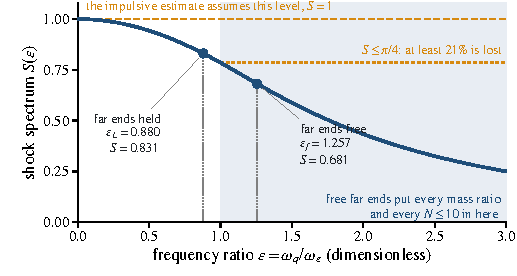
\includegraphics[width=\columnwidth]{fig_shock_spectrum}
  \caption{Half-sine shock spectrum $S(\varepsilon)$: the peak response to the pulse relative to the same impulse delivered instantly; \eqref{eq:imp} assumes $S=1$. Held far ends put the testbed at $\varepsilon_L=0.880$, $S=0.831$; free far ends force $\varepsilon_f\ge1$, so $S\le\pi/4$ for $N\le10$, and put the testbed at $\varepsilon_f=1.257$, $S=0.681$.}
  \label{fig:spectrum}
\end{figure}

The impulsive regime needs $\varepsilon_q\to0$, but with free far ends the neighbor mode is never slower than the pulse (Fig.~\ref{fig:spectrum}). The held case shows why \eqref{eq:imp} cannot be rescued by choosing the masses: $\varepsilon_L^2=(N-1)m_A/(m_A+m_L)$ is small, and the contact nearly impulsive, only when $m_A\ll m_L/(N-1)$, whereas held far ends require $\omega_f\approx\omega_L$, that is $m_A\gg m_L/(N-1)$. The two hypotheses demand opposite mass ratios, and the testbed, with $m_A/m_L=0.24$ against $1/(N-1)=0.25$, satisfies neither. Removing them one at a time, the finite pulse costs 17\% of \eqref{eq:imp}; the recoil of the far ends removes a further 43\% of what remains, and damping and drag 21\% of the rest, while the pulse shape assumed in Theorem~\ref{thm:closedform} changes the result by 1--2\%.

\subsection{Self-Consistent Contact Across Mass Ratios}\label{sec:selfconsistent}

We integrate \eqref{eq:model} with its unilateral force (adaptive RK4(5), relative tolerance $10^{-10}$, maximum step $\pi/(800\omega_e)$); with the prescribed pulse instead, this reproduces \eqref{eq:closedform} to six digits. For five cables the half-sine law is within $1.7$\% of the undamped self-consistent ratio for $m_A/m_L\le1$; the latter rises with vessel mass while far-end recoil dominates and falls once the lengthening contact does, with a secondary rise beyond $m_A/m_L\approx5$ (Fig.~\ref{fig:massratio}). We evaluate it on a 31-point logarithmic grid of $m_A/m_L$ over $[10^{-1.5},10^{1.5}]$ and refine the grid maximum by a bounded Brent search to $10^{-3}$. For $N=5$ this gives $\rho^\star=0.367$ at $m_A/m_L=1.41$, a numerical maximum, not a proof; by Corollary~\ref{cor:threshold}, no snap with $\bar T_{\mathrm p}<\Tn/\rho^\star\approx2.73\Tn$ slackens a neighbor in the undamped collinear model. For $N=3$--$8$ (Table~\ref{tab:worst}), every maximum lies more than a decade inside the interval and $(N-1)\rho^\star$ decreases monotonically from $1.54$ to $1.42$; whether this reflects a bound $\rho^\star\lesssim C/(N-1)$ is open, and for $N=2$ the search gives $\rho^\star=1.41$ at $m_A/m_L=4.0$.
\begin{figure}[t]
  \centering
  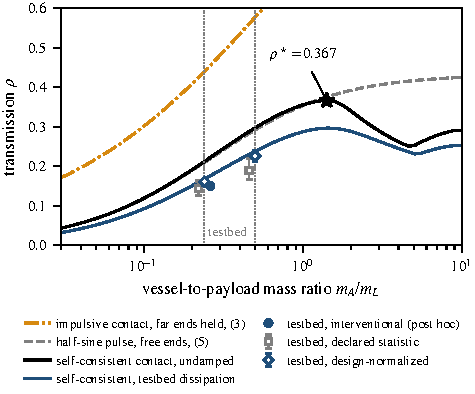
\includegraphics[width=\columnwidth]{fig_massratio}
  \caption{Five-cable transmission versus mass ratio. The undamped self-consistent contact has a numerical interior maximum $\rho^\star=0.367$ (star); the half-sine law tracks it for $m_A/m_L\le1$. Testbed markers, for the nominal cell of Section~\ref{sec:test} and its paired cell at $m_A=1250$\,kg: the recorded-geometry statistic (squares) and the design-normalized statistic (diamonds), both with seed intervals, the latter post hoc at $0.24$ and the declared primary of the second-mass test at $0.50$; and, at $0.24$, the post hoc interventional swing (circle).}
  \label{fig:massratio}
\end{figure}

\begin{table}[t]
  \caption{Largest Undamped Self-Consistent Transmission in the Mass-Ratio Search}
  \label{tab:worst}
  \centering
  \begin{tabular}{ccccc}
    \toprule
    $N$ & $m_A/m_L$ at max & $\rho^\star$ & $1/\rho^\star$ & $(N-1)\rho^\star$ \\
    \midrule
    3 & 2.67 & 0.770 & 1.30 & 1.54 \\
    4 & 1.94 & 0.501 & 2.00 & 1.50 \\
    5 & 1.41 & 0.367 & 2.73 & 1.47 \\
    6 & 1.11 & 0.289 & 3.46 & 1.45 \\
    7 & 0.92 & 0.239 & 4.19 & 1.43 \\
    8 & 0.78 & 0.203 & 4.92 & 1.42 \\
    \bottomrule
  \end{tabular}
\end{table}

\subsection{Dissipation and Stiffness}\label{sec:dissipation}

With the testbed's cable damping and drag (Table~\ref{tab:plant}), the self-consistent ratio is $0.167$ and the half-sine ratio $0.165$; the latter coincides to six digits with the planar forecast committed for the test of Section~\ref{sec:test}. By Proposition~\ref{prop:similarity} the stiffness enters only through the dissipation numbers, which yields two predictions. First, quartering and quadrupling $k$ moves $\rho$ from $0.139$ to $0.184$ under the half-sine pulse and from $0.140$ to $0.186$ self-consistently, increases of $0.045$ and $0.046$, whereas every undamped law, \eqref{eq:imp} and \eqref{eq:closedform} included, predicts none. Second, the swing's extremum, which Lemma~\ref{lem:spectrum} places at $2\pi/((1+\varepsilon_f)\omega_e)=149$\,ms without dissipation and which then scales as $k^{-1/2}$, arrives earlier with dissipation and scales more weakly: at $k/4$, $k$ and $4k$ the model places it at $205$, $125$ and $69$\,ms self-consistently and at $250$, $135$ and $71$\,ms under the half-sine pulse. Only the half-sine values of the first prediction were committed before the campaign, as the planar forecast; the self-consistent and timing values were computed after the measurements of Section~\mbox{\ref{sec:stiffness}}.

\section{Simulation of a Multibody Fleet}\label{sec:test}

We test the collinear predictions on a planar Drake model \cite{tedrake2019drake} of five tugs and one payload (Table~\ref{tab:plant}). The payload is a regular pentagon of circumradius $4$\,m with bow attachments spanning $\pm31.7^\circ$, and each vessel attaches $1.5$\,m astern of its center; parallel cells keep the nominal chords parallel, fan cells spread them over $\pm0.55$\,rad. Each vessel holds its steady-tow thrust open-loop and runs a $50$\,Hz heading loop, proportional in heading error with a cable-bearing trim term; every body receives first-order autoregressive weather with $8$\,s memory. The plant is integrated at $0.5$\,ms. An isolated vessel--payload refinement passes a $0.5$\% energy-envelope criterion at $0.5$\,ms with little margin ($0.47$\%; $0.95$ and $0.23$\% at $1.0$ and $0.25$\,ms) and so selected $0.25$\,ms; the campaign uses $0.5$\,ms for cost, at which the five-vessel engagement peak lies within $0.08$\% of its $0.25$\,ms value. As the cable force is explicit, the error scales with $\omega_e h$ for step $h$, so the $4k$ cells sit at the nominal $1.0$\,ms level. A check declared before its runs re-ran the nominal and $4k$ cells on all 22 seeds at $0.25$\,ms, re-integration of Section~\ref{subsec:magnitude} included: the declared and design-normalized statistics and the interventional swing moved by at most $0.006$ and its lag by under $1$\,ms, each change inside its paired interval and below the half-width of its seed interval.

\begin{table}[t]
  \caption{Testbed Parameters}
  \label{tab:plant}
  \centering
  \setlength{\tabcolsep}{3.4pt}
  \renewcommand{\arraystretch}{0.96}
  \begin{tabular}{llr}
    \toprule
    Quantity & Symbol & Value \\
    \midrule
    Payload mass, drag & $m_L$, $c_L$ & $2500$\,kg, $5500$\,N\,s/m \\
    Vessel mass, drag & $m_A$, $c_A$ & $600$\,kg, $350$\,N\,s/m \\
    Cable stiffness, damping & $k$, $c$ & $1.7\!\times\!10^{5}$\,N/m, $1800$\,N\,s/m \\
    Cable rest length & $L$ & $12$\,m \\
    Payload, vessel yaw inertia & $I_L$, $I_A$ & $2.0\!\times\!10^{4}$, $500$\,kg\,m$^2$ \\
    Payload, vessel yaw drag & & $2.0\!\times\!10^{4}$, $800$\,N\,m\,s \\
    Heading gain (nominal, doubled) & & $500$, $1000$\,N\,m/rad \\
    Cable-bearing trim gain & & $100$\,N\,m \\
    Steady thrust (parallel cells) & $F_T$ & $1.32\,T_0$ \\
    Weather std, payload/vessel & $\sigma_W$ & $3.5$, $0.7$\,kN \\
    Weather memory & $\tau_W$ & $8$\,s \\
    Engagement, payload modes & $\omega_e$, $\omega_L$ & $18.7$, $16.5$\,rad/s \\
    \bottomrule
  \end{tabular}
\end{table}

The campaign has sixteen cells: ten parallel cells spanning $T_0\in\{0.6,1.0,1.4,1.8\}$\,kN, weather intensity $0.5$ or $1$ (Table~\ref{tab:plant} lists intensity 1), and nominal or doubled heading gain; two stiffness cells at $k/4$ and $4k$; and four fan cells. Each cell runs the same 22 seeds, of which 20 are scored; the two pilot seeds, reserved by the declaration for fitting, fit only the neighbor-margin law of the slack-onset test cited in Section~\ref{sec:consequences}. Re-engagements of one cable within $2$\,s of its first form one event, and a scored observation pairs that first re-engagement, with $\Tp\in[T_0,4T_0]$ and all other cables taut, with one neighbor. Drops are read over one engagement period $P=2\pi\sqrt{\mu/k}$, $\mu=m_Am_L/(m_A+m_L)=484$\,kg. Intervals are 95\% bootstraps over whole seeds, with 2000 replicates unless a caption states otherwise.

\subsection{Forecast, Protocol, and Evidence Status}
\label{subsec:forecast}

We committed the forecast and every pass criterion to a hashed declaration \cite{nosek2018preregistration,siepe2024simulation} before launching the campaign and before any neighbor-tension drop had been computed. Ten of the sixteen cells (220 of 352 runs) re-simulate, bit for bit, an earlier campaign on the same seeds, whose stored records (slack-event times and peaks, 1\,Hz tension samples) cannot yield the declared statistic; the forecast has no fitted input. The forecast $R_{ij}$ is the peak tension reduction in cable $i$ per unit half-sine peak applied through cable $j$, from a 34-state translation-invariant linearization of the closed-loop planar fleet about steady tow that retains drag, cable damping, and heading control; the snapping cable contributes only its pulse wrench, and the outputs are $k\,\delta e_i+c\,\delta\dot{e}_i$. Central-difference Jacobians use a step of $10^{-5}$ per reduced coordinate; steps of $10^{-4}$ and $10^{-6}$ change every $R_{ij}$ by less than $10^{-4}$\%.

The declared (pre-registered) window statistic divides the measured tension reduction by $\Tp g_{ij}$, where $g_{ij}$ is the $(i,j)$ entry of $G=(2k/(\omega_L\omega_e))W^\top M_L^{-1}W$ (Section~\ref{sec:model}) divided by \eqref{eq:imp}. At the design geometry of the parallel cells the off-diagonal $g_{ij}$ range from $0.50$ to $1.23$; the statistic instead evaluates $g_{ij}$ at the recorded geometry of each event, where it can approach or cross zero ($g_{ij}\le0$ for $14$--$39$\% of a cell's scored observations). The cell forecast is the median of $R_{ij}/g_{ij}$ over the 20 ordered pairs at the design geometry: $0.165$ in the ten parallel cells at nominal stiffness, $0.139$ and $0.184$ at the stiffness extremes, and $0.176$ in the fan cells. Table~\ref{tab:evidence_status} gives the status of each analysis, that is, when it was specified relative to the data it evaluates.

\begin{table*}[t]
\caption{Evidence Status and Principal Outcomes}
\label{tab:evidence_status}
\centering
\footnotesize
\setlength{\tabcolsep}{3pt}
\renewcommand{\arraystretch}{1.05}
\begin{tabular}{>{\raggedright\arraybackslash}p{2.2cm} >{\raggedright\arraybackslash}p{2.2cm} >{\raggedright\arraybackslash}p{2.9cm} >{\raggedright\arraybackslash}p{5.6cm} >{\raggedright\arraybackslash}p{3.4cm}}
\toprule
\textbf{Analysis} & \textbf{Status} & \textbf{Prediction or benchmark} & \textbf{Observed outcome} & \textbf{Interpretation} \\
\midrule
Impulsive band & Pre-registered & No cell in $[0.2,0.9]$ & None enters; cell medians $0.054$--$0.173$ & Rejects the rigid-impact magnitude \\
Small-peak accuracy & Pre-registered & Ratio to forecast within $\times1.5$, $\Tp<2.3T_0$ & $0.83$--$1.48$ in all 15 evaluable cells & Forecast within declared factor \\
Stiffness trend & Pre-registered & $+0.045$ from $k/4$ to $4k$ & $+0.036$ [$+0.015,+0.058$] & Supports dissipative dependence \\
Pairwise ranking & Pre-registered & Pair order of $R_{ij}$ & Met in 2 of 15 evaluable cells & No pairwise claim \\
Fixed dissipation & Declared addendum & No change, $\gamma$'s fixed & Declared statistic $+0.038$ [$+0.013,+0.060$], a failure; swing (no rule) $+0.007$ [$-0.002,+0.019$] & Statistic responds to geometry; swing flat \\
Second mass ratio & Declared addendum; 18 of 20 seeds blind & Design-normalized $+0.070$ & $+0.065$ [$+0.051,+0.081$]; blind $+0.058$ [$+0.047,+0.081$] & Supports the rise at a second point \\
Magnitude & Post hoc & Committed $0.165$ & Interventional $0.148$ [$0.143,0.154$] ($0.95\times$ forecast per observation; integrator check failed); background-subtracted $0.093$; design-normalized nominal $0.161$ [$0.151,0.167$] & Approximate population magnitude, not a bound \\
\bottomrule
\end{tabular}
\end{table*}

\subsection{Magnitude}\label{subsec:magnitude}

\begin{figure}[t]
  \centering
  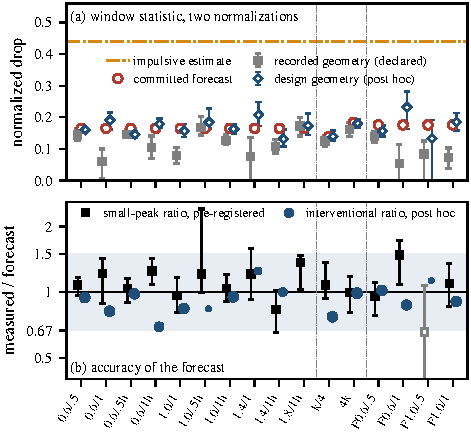
\includegraphics[width=\columnwidth]{fig_cells}
  \caption{Transmission in sixteen cells, labeled by $T_0$ in kN and weather intensity (h: doubled heading gain; F: fan; $k/4$, $4k$: stiffness cells). (a) Declared recorded-geometry statistic (squares) and post hoc design-geometry reading (diamonds), with seed intervals, against the committed forecast (circles). (b) Measured over forecast: pre-registered small-peak ratio (squares, seed intervals; open: unscored cell) and post hoc interventional ratio (circles, area growing with observation count); the band is the declared factor $1.5$.}
  \label{fig:cells}
\end{figure}

The declared statistic stays below the impulsive band $[0.2,0.9]$ in every cell (Fig.~\ref{fig:cells}a) but below the forecast in 14 of 16. On the 3008 re-integrated observations introduced below, an additive background floor ($0.057\Tp$ in time-shifted windows against $0.154\Tp$ at snaps) would raise it; the offset comes instead from the recorded-geometry normalizer, which approaches or crosses zero at re-engagement, and from background motion of either sign inside the window, which can mask the snap response (8\% of those observations record no drop). On them, the drop is $0.80$ times the forecast at the recorded normalizer and $0.99$ at the design normalizer. Applied post hoc, the design normalizer moves the cell medians to $0.132$--$0.232$, putting two cells ($0.208$, $0.232$) inside $[0.2,0.9]$, and the nominal cell ($T_0=0.6$\,kN, intensity $0.5$) from $0.144$ [$0.127,0.163$] to $0.161$ [$0.151,0.167$]; these readings keep the background. For peaks below $2.3T_0$, the pre-registered ratio to the forecast lies within the declared factor $1.5$ in all 15 evaluable cells ($0.83$--$1.48$, Fig.~\ref{fig:cells}b); the fan cell at $T_0=1.0$\,kN, intensity $0.5$, has 12 such observations, below the declared minimum of 20 (unscored ratio $0.66$).

A post hoc estimator, added after the pre-registered verdicts, removes the background: it re-integrates each snap from the recorded state $0.5$\,s before re-engagement under the recorded weather, once as recorded and once without the snapping cable's force, and takes the largest tension difference within one engagement period, on a $10$\,ms grid, per unit $\Tp$ (the interventional swing). It uses a separate $0.5$\,ms semi-implicit Euler model with constant thrust and headings replayed from the record, so the heading loop is not simulated. Its pre-registered check against the record failed on two criteria: other cables' slack onsets over $3$\,s were reproduced for $94.9$\% of 9646 re-engagements against $95$\% ($61$\% in the $4k$ cell, at least $93.8$\% elsewhere), and one grazing contact re-engaged $5.2$\,ms late against a $5$\,ms limit; the median timing error is $6\,\mu$s and the 95th-percentile peak error $0.35$\%. The 3008 observations cover all 22 seeds of four cells and only the two pilot seeds of eleven others (624 from pilots; 2800 at $T_0=0.6$\,kN). Their median swing is $0.148\Tp$ [$0.143,0.154$]; per observation it is $0.95$ times the forecast, and cell medians range from $0.69$ to $1.25$ times it. Subtracting each observation's own time-shifted drop instead (2928 observations with a background window) gives $0.093\Tp$, a lower bound, since background and snap do not add inside a minimum; the gap between the two readings is the width of this measurement.

\begin{figure}[t]
  \centering
  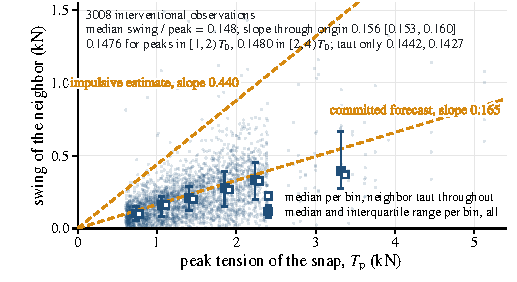
\includegraphics[width=\columnwidth]{fig_swing_vs_peak}
  \caption{Post hoc interventional swing versus snap peak for 3008 observations: medians and interquartile ranges per bin (filled) and medians for the 2766 observations whose neighbor stays taut (open). The through-origin slope is $0.156$ [$0.153,0.160$] (400 bootstrap replicates), versus $0.165$ forecast and $0.440$ impulsively.}
  \label{fig:swingpeak}
\end{figure}

The interventional ratio is $0.1476$ for $\Tp\in[T_0,2T_0)$ and $0.1480$ for $\Tp\in[2T_0,4T_0)$ (Fig.~\ref{fig:swingpeak}), and $0.1442$ and $0.1427$ for neighbors that stay taut, each with a seed interval of $\pm0.005$--$0.008$. They are consistent with, but do not prove, the amplitude invariance of Proposition~\ref{prop:similarity}.

\subsection{Parameter Dependence and Unloading}\label{sec:stiffness}
\begin{figure}[t]
  \centering
  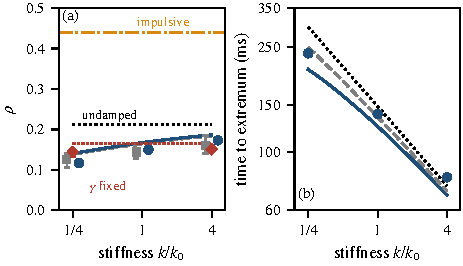
\includegraphics[width=\columnwidth]{fig_stiffness}
  \caption{Stiffness test in the nominal cell. (a) Declared statistic (squares, seed intervals) and post hoc interventional swing (circles) against the dissipative self-consistent (solid) and half-sine (dashed, the committed forecast) models, the undamped law (dotted), and the impulsive estimate (dash-dotted); diamonds: swing on the fixed-dissipation control cells against their flat forecast (red dotted); the control's declared statistic, $0.116$ to $0.154$, which fails that forecast, is not drawn. (b) Time from the snap to the swing's extremum against the same models.}
  \label{fig:stiffness}
\end{figure}

Between $k/4$ and $4k$ the declared statistic rises from $0.125$ to $0.161$, $+0.036$ [$+0.015,+0.058$] over 20 paired seeds, against $+0.045$ predicted and zero from the undamped laws (Fig.~\ref{fig:stiffness}a), the outcome declared as confirming. The median recorded geometry factor is flat in this pair ($0.77$ to $0.78$), so the rise is in the drop itself ($0.135$ to $0.168$ per unit peak). The interventional extremum occurs at $236$, $139$, and $80$\,ms for $k/4$, $k$, and $4k$ (Fig.~\ref{fig:stiffness}b), a ratio of $2.96$ against $2.99$ for the self-consistent model, $3.5$ for the half-sine pulse, and $4$ undamped. That agreement is post hoc: the model times were computed after the measurements, the lags lie on a $10$\,ms grid, and the $k/4$ value rests on 13 snaps from the two pilot seeds.

A control declared before its runs scales $c$, $c_L$, $c_A$ by $\sqrt{k/k_0}$ while varying $k$ (nominal $k_0$), holding $\gamma$, $\gamma_L$, $\gamma_A$ and the linearized forecast fixed at $0.165$. By its declared rule it fails: the declared statistic rises by $+0.038$ [$+0.013,+0.060$]. The rise comes from the normalizer: as the scaled drag changes the shape the fleet holds at re-engagement, the share of observations with $g_{ij}\le0$ falls from $27$ to $16$\% (median $g_{ij}$ $0.69$ to $0.85$), while the drop per unit peak falls from $0.162$ to $0.142$. The interventional swing, declared as a second statistic without an outcome rule, carries neither background nor normalizer and is flat, $0.144$ to $0.151$, $+0.007$ [$-0.002,+0.019$], against $0.117$ (13 pilot snaps) to $0.173$ in the pre-registered pair; its lag ratio is $4.6$ against $4.0$ for the model. On the reading that isolates the transmission, stiffness enters through dissipation, as Proposition~\ref{prop:similarity} states; the declared statistic is also sensitive to the fleet's geometry.

\noindent\textit{Pair structure.}
The post hoc swing improves the rank correlation with $R_{ij}$ in the four fully re-integrated cells ($0.76$, $0.83$, $0.95$ in the parallel cells and $0.47$ in the fan, against $0.24$, $0.21$, $0.58$, $0.31$ for the window drop on the same observations), but the spread of its pair medians within a cell is only $0.054$--$0.067$, against $0.125$--$0.189$ for $R_{ij}$.

\noindent\textit{A second mass ratio.}
A later addendum raised $m_A$ from $600$ to $1250$\,kg ($m_A/m_L=0.50$), for which the collinear model predicts $0.167\to0.238$, printed before the run, and the planar linearization $0.165\to0.234$. It was written after a four-seed pipeline check whose two scored seeds were seen, and its primary statistic is the post hoc design-normalized reading. That statistic rises by $+0.065$ [$+0.051,+0.081$] against $+0.070$ predicted, and by $+0.058$ [$+0.047,+0.081$] on the 18 unseen seeds. The declared secondary statistic, at the recorded geometry, rises by $+0.046$ [$+0.022,+0.073$] ($0.144\to0.189$), and by $+0.038$ [$+0.017,+0.068$] on the unseen seeds; no rule was declared for it.

\noindent\textit{Unloading criterion.}
\begin{figure}[t]
  \centering
  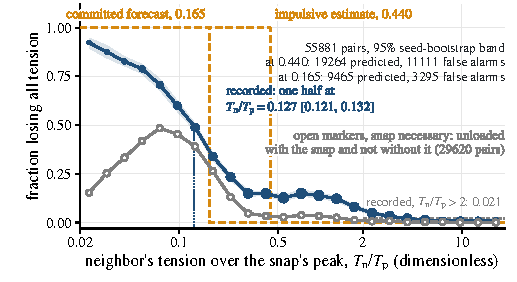
\includegraphics[width=\columnwidth]{fig_threshold_curve}
  \caption{Empirical analog of Corollary~\ref{cor:threshold} over 55\,881 (parent, taut neighbor) pairs. Each candidate $\rho$ is a threshold on $\Tn/\Tp$ (steps); the blue curve (marker area growing with pair count) is the recorded unloading probability with a 400-replicate seed band, crossing one-half at $0.127$ [$0.121,0.132$]. The gray curve (open markers), over 29\,620 re-integrated pairs, is the fraction unloaded in the recorded branch but not the counterfactual one; the dotted level, $0.021$, is the recorded rate at $\Tn/\Tp>2$.}
  \label{fig:threshold}
\end{figure}
Fig.~\ref{fig:threshold} scores $\Tn/\Tp$ over 55\,881 pairs of a declustered parent and a taut neighbor; $19.2$\% unload, and $45.8$\% of the 18\,116 with $\Tp>4T_0$. It is an analog rather than a test of Corollary~\ref{cor:threshold}, which uses $\bar T_{\mathrm p}$ where the figure uses the recorded $\Tp$; the two differ when a neighbor unloads early, as 41\% of unloaded neighbors do within $60$\,ms, near or before the parent's peak. The unloading probability crosses one-half at $0.127$ [$0.121,0.132$]; as classifiers, $\rhoimp=0.440$ recovers 8153 of 10\,735 unloadings with 11\,111 false alarms, and $0.165$ recovers 6170 with 3295. The gray curve counts a neighbor whose elongation crosses zero within $3$\,s in the recorded branch but not in the counterfactual one, the snap as a necessary cause; since the integrator's pre-registered check failed, the declaration requires these counts to be reported as untrusted. It peaks near one-half for $\Tn/\Tp\in[0.05,0.15]$ and is $0.004$ for $\Tn/\Tp>2$ ($0.018$ over all $\Tn/\Tp>0.44$, where neither candidate predicts unloading). The planar transition is therefore population-level, not a deterministic bound on every pair.

\section{Consequences, Limitations, and Conclusion}\label{sec:consequences}

On the nonlinear fleet, the collinear theory and the simulation agree on the magnitude and on its stiffness and mass dependence, but not on the distribution over pairs. The post hoc magnitudes, $0.148$ by intervention and $0.161$ by design normalization, lie within about 10\% of the committed $0.165$, above the background-subtracted bound $0.093$ and far below the impulsive $0.44$.

By Corollary~\ref{cor:threshold}, a snap unloads a neighbor at $\Tn$ once $\bar T_{\mathrm p}$ reaches $\Tn/\rho$: at pretension, $2.3T_0$ for the impulsive model, $6.1T_0$ and $6.8T_0$ for the committed and interventional magnitudes, and $10.8T_0$ for the background-subtracted bound. These are extrapolated scale estimates, not design bounds: the magnitude sample stops at $4T_0$, and zero tension censors the taut response. Neighbors of scored snaps carry per-cell median tensions of $1.1$--$2.0T_0$, so $\rho\approx0.15$ places isolated unloading near $7$--$14T_0$, several times the median parent peak of $2.5T_0$; yet one parent snap in five exceeds $7T_0$. Of the 10\,735 recorded unloadings in Fig.~\ref{fig:threshold}, 69\% struck neighbors at or above pretension and 60\% followed peaks above $7T_0$; the counterfactual counts, reported as untrusted, sharpen this to 79\% and 82\% of the 4336 unloadings for which the snap was a necessary cause (78\% and 76\% after reweighting for the re-integration sampling). Snap-driven unloading on this testbed thus comes mainly from the upper tail of snap peaks acting on normally loaded neighbors, not from neighbors near slack. The finite-contact law should not be read as bounding how readily slack spreads: the pre-registered test that turned $R_{ij}$ and the neighbor margins into predicted slack onsets failed, under-predicting them in all 16 cells by factors of $0.39$--$0.80$ ($0.65$--$0.98$ against a post hoc target of neighbors taut at the snap). Cable severance, which redistributes steady tension rather than transmitting a snap, is treated in \cite{hajieghrary2026passive}.

The conclusions have three limits. The exact theory is collinear with lumped cables, whereas distributed lines carry the snap as a wave, and whether lever arms and yaw can raise a pair above the collinear worst case is open. The planar testbed has linear drag and no hull contact, and the interventional estimator (whose integrator failed its pre-registered check), the design normalization, and the timing comparison are post hoc. Two mass ratios, $0.24$ and $0.50$, test the rising branch of Fig.~\ref{fig:massratio}; the interior maximum near $1.4$ is numerical, not measured or proved. Measuring it, and the pairwise distribution of $\rho$ with its upper tail, on the planar fleet is future work.

\noindent\textit{Data, code, and pre-registration.} The declaration record (SHA-256 prefix \texttt{fc26c18c14b97b04}) fixed the plan, cells, tests, pass criteria, and forecast before the campaign, pins the digests of the plan, forecast, theory document, modules, and inputs it uses, and was never edited. Of eight dated addenda, one records a reducer-crash fix, four record post hoc sensitivities, corrections, or reporting constraints that change no declared test, threshold, population, or rule, and three declare the fixed-dissipation control and the step-size check before their runs and the second mass ratio after a four-seed pipeline check. The declarations, addenda, run records, analysis code, and figure scripts are available from the authors.


\bibliographystyle{IEEEtran}
\bibliography{refs}

\end{document}
